\documentclass{beamer}
\usepackage[utf8]{inputenc}
\usepackage{amssymb}
\usepackage{amsmath}
\usepackage{dsfont}
\usepackage{stmaryrd}
\usepackage{graphicx}
\usepackage{animate}

\graphicspath{{./images/}{./images/video/}}

\title{Optimisation stochastique, (RJ)MCMC\\ et applications g\'eospatiales}
\author{}
\institute{IGN}
\date{2015}

\begin{document}
\frame{\titlepage}
 
\begin{frame}
\frametitle{Contexte}
\begin{itemize}
\item La recherche de l'IGN a souvent des probl\`emes d'optimisation (comme tout le monde)
\item D\'eveloppement d'outils \emph{sp\'ecifiques} (g\'en\'eralisation carto)
\item D\'eveloppement d'un biblioth\`eque plus \emph{g\'en\'erique}
\end{itemize}
\end{frame}

\begin{frame}
\frametitle{La \emph{libRJMCMC}}
Elle propose~:
\begin{itemize}
\item un \'echantillonneur RJMCMC
\item un recuit simul\'e (ou parallel tempering)
\item des exemples et des applications
\end{itemize}
Plusieurs impl\'ementations~:
\begin{itemize}
\item C++ \small[\url{http://github.com/IGNF/librjmcmc}], license CeCILL-B
\item Java \small[\url{http://github.com/IGNF/librjmcmc4j}], license XXX
\item Scala \small[\url{http://github.com/IGNF/librjmcmc4s}], license XXX
\end{itemize}
Le tout sous licence libre.
\end{frame}

\section{Applications}

\begin{frame}
\frametitle{Reconstruction d'emprises de bâtiments rectangulaires}
\emph{Le probl\`eme~:} 
\begin{itemize}
\item Détecter des emprises de bâtiments sur un MNS satellite.
\end{itemize}
\emph{Les concepts~:}
\begin{itemize}
\item MPP~:  $\mathcal{C} = \cup_{n}\mathcal{B}^n$\\
avec $\mathcal{B}=[0,W]\times[0,H]\times[-S,S]^2\times[1/R,R] \subset  \mathds{R}^{5}$
\item Noyaux~: Naissance/mort, translation d'une arête, rotation/homothétie autour d'un coin, Division/Fusion
\item Processus de référence~:
\begin{itemize}
\item Processus de poisson sur $n$
\item Uniforme sur $\mathcal{B}$
\end{itemize}
\item \'Energie~: $E = \sum_i E_1(x_i) + \sum_{i<j} E_2(x_i,x_j)$
\begin{itemize}
\item $E_1(x_i)=\alpha_{0} - E_{data}(x_i)$ avec $\alpha_{0}>0$ ;
\item $E_2(x_i,x_j) = surface(x_i \cap x_j)$.
\end{itemize}
\end{itemize}
\end{frame}

\begin{frame}
\frametitle{Extraction des marquages aux sols}
\emph{Le probl\`eme~:} 
\begin{itemize}
\item Détecter différents types de marquages sur une ortho-image.
\end{itemize}
\emph{Les concepts~:}
\begin{itemize}
\item MPP~:  $\mathcal{C} = \cup_{n}\mathcal{B}^n$\\
avec $\mathcal{B}=\{1...\vert \mathcal{L}\vert\}\times [0,W]\times[0,H]\times[-\pi,\pi]\times[\lambda-\epsilon,\lambda + \epsilon] \subset  \mathds{R}^{5}$
\item Noyaux~: Naissance/mort, translation, rotation, changement d'échelle, changement de type. 
\item Processus de référence~:
\begin{itemize}
\item Processus de poisson sur $n$
\item \color{red}{Data\&Model driven}
\end{itemize}
\item \'Energie~: $E = \sum_i E_1(x_i) + \sum_{i<j} E_2(x_i,x_j)$
\begin{itemize}
\item $E_1(x_i)=\alpha_{0} - E_{data}(x_i)$ avec $\alpha_{0}>0$ ;
\item $E_2(x_i,x_j) = \frac{(x_i \cap x_j)}{min(surface(x_i),surface(x_j)}$.
\end{itemize}
\end{itemize}
\end{frame}
%
\begin{frame}
\frametitle{Extraction des marquages aux sols}
\emph{R\'esultats~:}
\begin{center}
\begin{figure}[ht]
\animategraphics[scale=0.5, controls]{12}{}{1}{92}
\end{figure}
sss
\end{center}
\end{frame}

\begin{frame}
\frametitle{Simplu3D}
\emph{Le probl\`eme~:}  Simulation des droits \`a batir
\begin{itemize}
\item Génération de configurations bâties pour évaluer l'influence des réglements des PLU
\end{itemize}
\emph{Les concepts~:}
\begin{columns}
\begin{column}{0.55\textwidth}
\begin{itemize}
\item MPP~:  $ \mathcal{C} =\cup_{n} \mathcal{B}^n$  avec $\mathcal{B}  \subset  \mathds{R}^{6}$
\item Noyaux~: Naissance/mort, translation, rotation, changement de dimension (longueur, largeur ou hauteur)
\end{itemize}
\end{column}
\begin{column}{0.45\textwidth}
 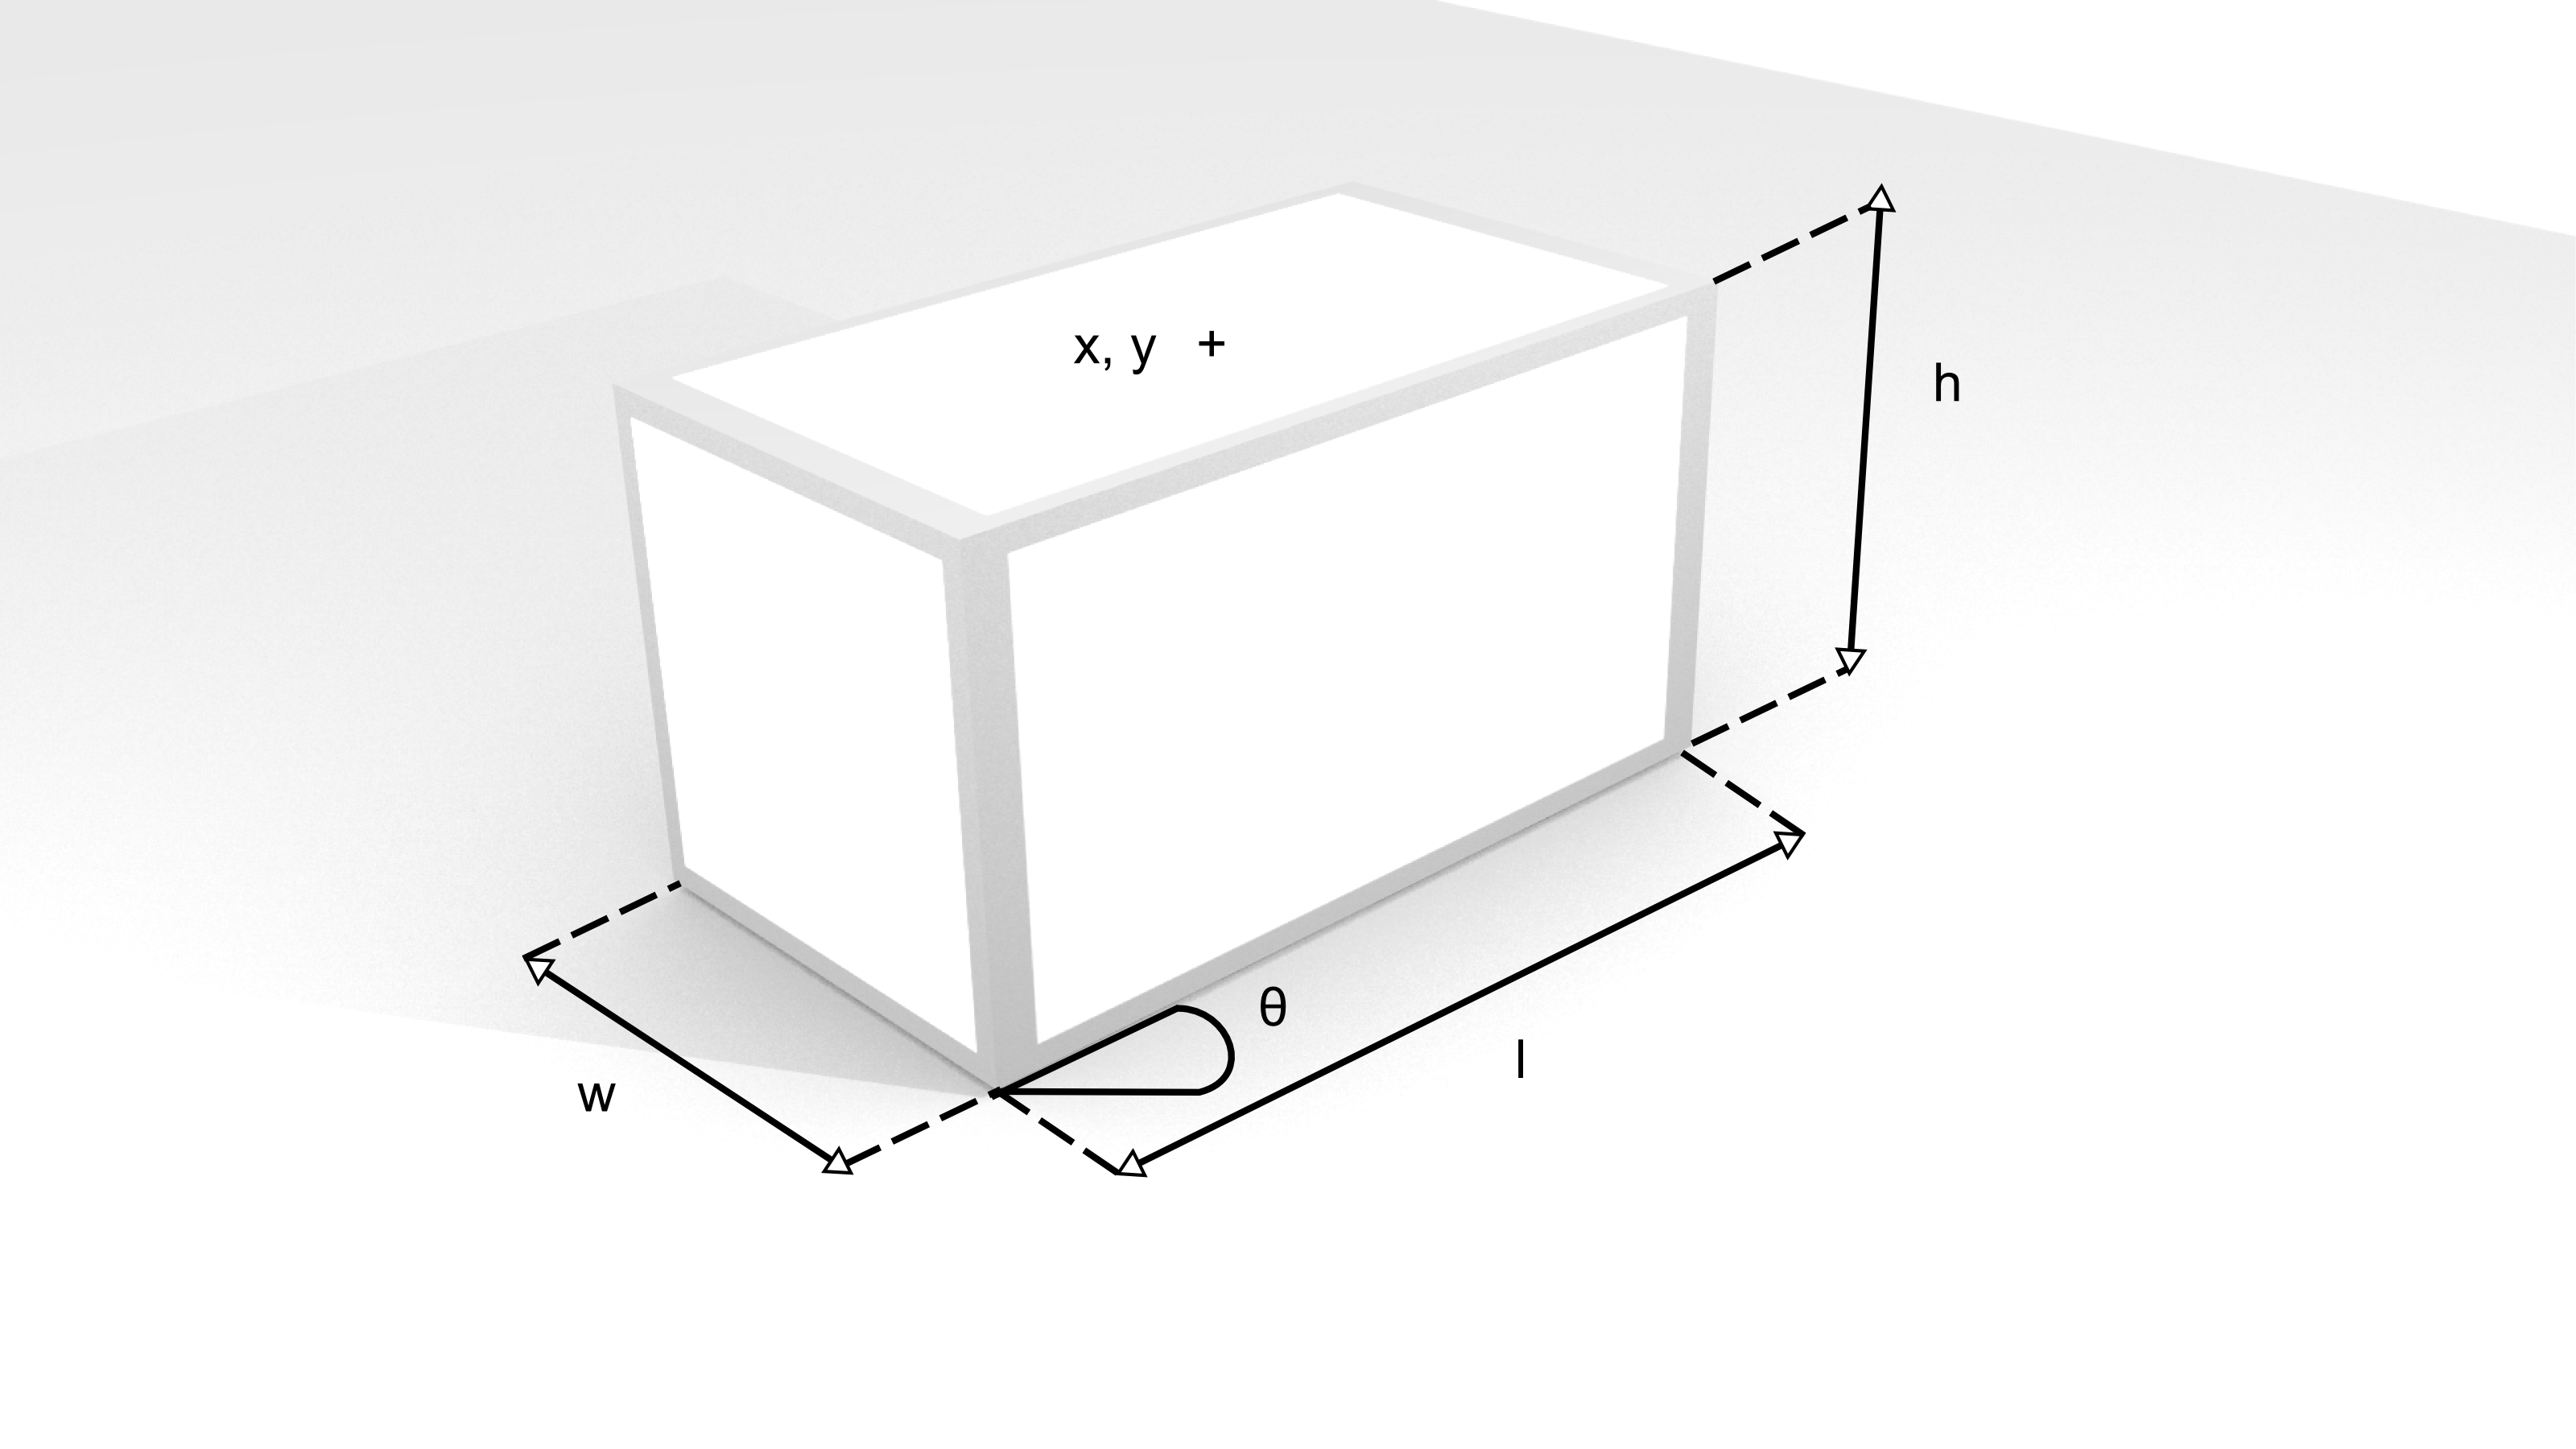
\includegraphics[width=\textwidth]{boiteFin.png}
\end{column}
\end{columns}
\begin{itemize}
\item Énergie~: $\mu = \mu_{unaire} + 2 \times \mu_{binaire}$
\begin{itemize}
\item $\tilde \mu_{unaire}(b \in \mathcal{B})=\alpha_{0} - volume(b)$ avec $\alpha_{0} \in \Re^{+*}$ ;
\item $\tilde \mu_{binaire}(b \in \mathcal{B}, b' \in \mathcal{B})) = volume(b \cap b')$.
\end{itemize}
\item Contraintes~:  $ \mathcal{S} = \mathcal{PLU} \cap  \mathcal{C}   $
\end{itemize}


\end{frame}

\begin{frame}
\frametitle{Simplu3D}
\emph{R\'esultats:}
 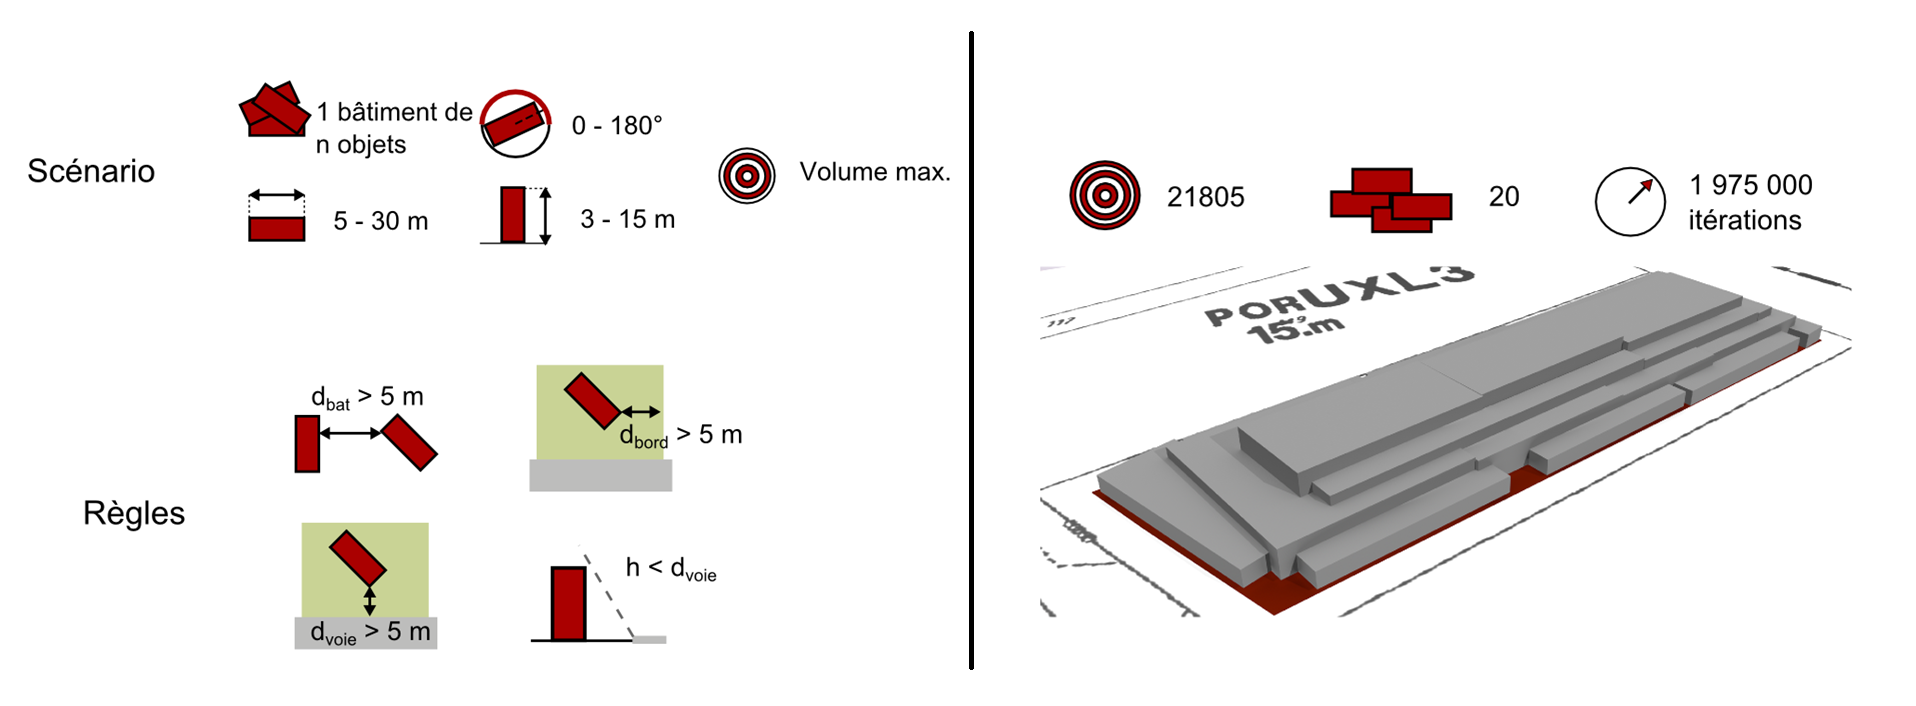
\includegraphics[width=\textwidth]{simplu3D1.png}
\end{frame}

\begin{frame}
\frametitle{Simplu3D}
\emph{R\'esultats:}
 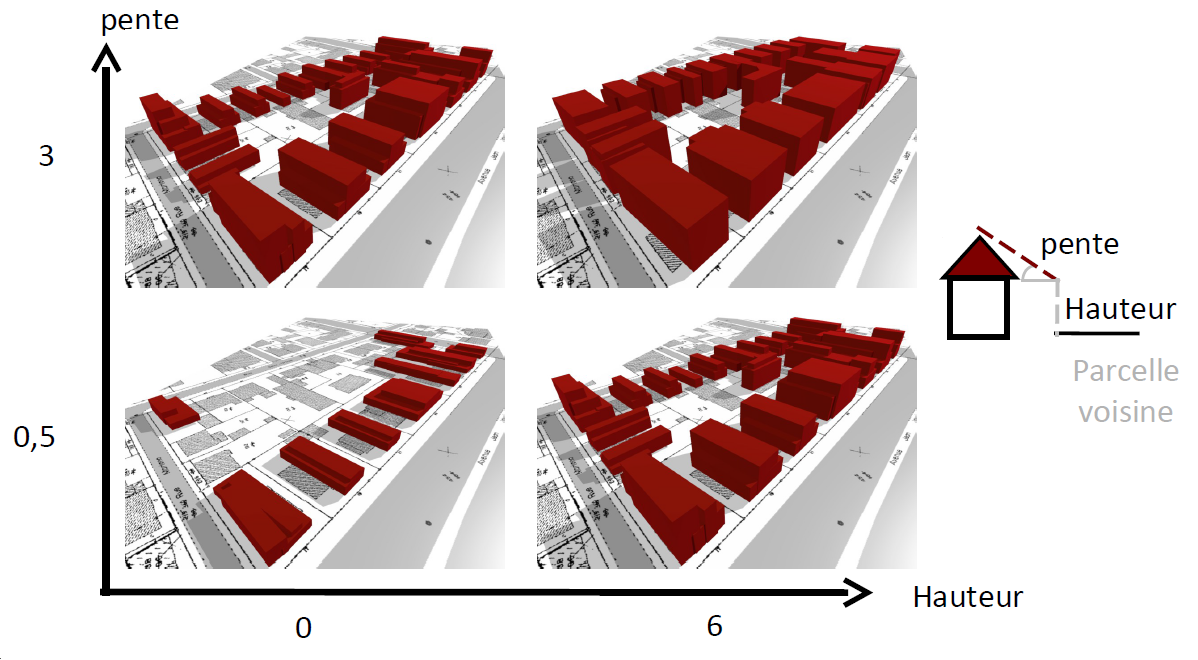
\includegraphics[width=\textwidth]{simplu3D2.png}
\end{frame}

\begin{frame}
\frametitle{Perspectives}
\emph{Parallelisation~:} 
\begin{itemize}
\item Distributed tempering
\item De l'espace de recherche -> passage à l'échelle
\item Openmole
\end{itemize}

\emph{Nouvelles applications~:} 
\begin{itemize}
\item Maillage simplifié (espace de recherche des triangulations)
\item ...
\end{itemize}
\end{frame}

\begin{frame}
\frametitle{Conclusion}
\begin{itemize}
\item Recherche reproductible
\item $\Rightarrow$ Appel à Contribution ?
\end{itemize}

\end{frame}


\end{document}
